Predicting election results in the US has been a popular news topic, as much as sports. Not only is the election itself seen as a race, forecasters compete with one another as a sport. The objective of the game is not to place balls into the rim or between goal posts. In this sport, the performance is measured as forecast error. 

Just as a pitcher may benefit from learning aerodynamics to develop better pitches, a election forecaster can improve their crafts by understanding the nature of unpredictability in elections. Election forecasters have come up with methods to improve, including development of random sampling in polling and survey weighting. The very nature of unpredictability remains a large mystery.

What influences unpredictability of elections? Does it change? By using national presidential and parliamentary elections among many OECD countries across multiple decades, \cite{nadeau_2019} found that the forecast error, measured by mean absolute error, stays consistent over multiple election cycles. We want to turn cross-national comparison into a cross-state comparison in the US. We want to examine phenomenon within one election cycle.

Forecast error based on models with vote-intention (poll) data reduces as the time of the poll gets closer to the election date. This result makes sense intuitively. It is easier to make a forecast about things that will happen in a week than things that will happen in 3 months. What other factors may explain forecast error and predictability of election result. 

In the context of the US presidential election, news media and campaigns often focus their eyes on swing states. Is it easier to predict election results in swing states than non-swing states? There are three mutually exclusive views on this. 

Systematically, election results in swing states are more predictable. This may arise because there are higher number and more accurate state polls. There are more attempts from pollsters to learn better on voter intention at these key battleground states. Figure 1 and Table 1 show that in the 2020 US presidential election cycle, there are more state polls among battleground states than the others.

The second view is that swing states results are harder to predict. There are more campaign efforts including TV, internet and billboard advertising as well as rallies and canvassing. This might mean that the volatility of voter intention is swing states is higher, making the prediction results less accurate.  

The third view is that there is no systematic difference between two types of states.


%Make sure to include [H] to place the figure in the text
\begin{figure}[H]
    \centering
    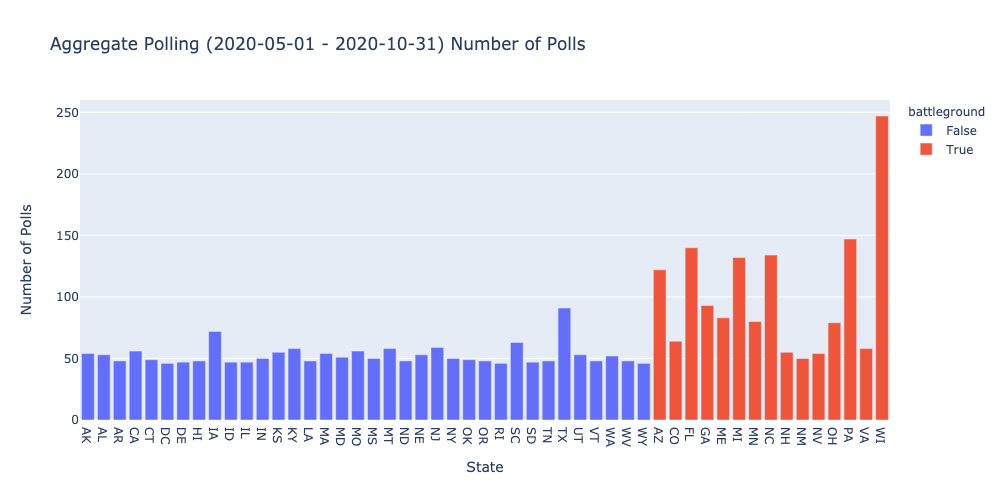
\includegraphics[height=20em]{figures/aggregate_polling_2020-05-01_-_2020-10-31_number_of_polls.png}
    \caption{}
    \label{fig:aggregate_polling_2020-05-01_-_2020-10-31_number_of_polls}
\end{figure}

\begin{table}[H]
\begin{table}
\centering
\caption{Aggregate Polling (2020-05-01 - 2020-10-31) Number of Polls}
\begin{tabular}{lr}
\toprule
 battleground &        mean \\
\midrule
        False &   52.666667 \\
         True &  102.533333 \\
\bottomrule
\end{tabular}
\end{table}

    \label{tab:aggregate_polling_2020-05-01_-_2020-10-31_number_of_polls}
\end{table}

As shown in \ref{tab:aggregate_polling_2020-05-01_-_2020-10-31_number_of_polls}, we see that there is more polling in battleground states than non-battleground states.\\

\begin{figure}[H]
    \centering
    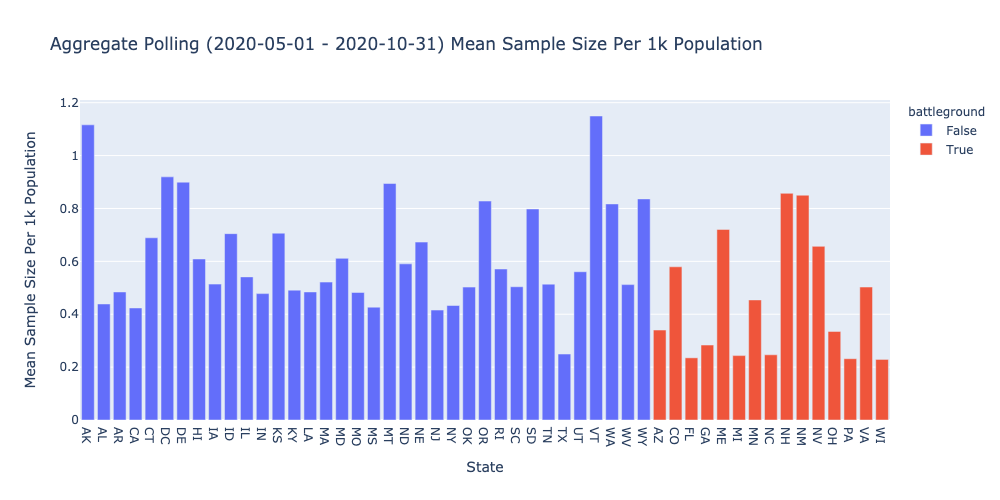
\includegraphics[height=20em]{figures/aggregate_polling_2020-05-01_-_2020-10-31_mean_sample_size_per_1k_population.png}
    \caption{}
    \label{fig:aggregate_polling_2020-05-01_-_2020-10-31_mean_sample_size_per_1k_population}
\end{figure}

\begin{table}[H]
\begin{table}
\centering
\caption{Aggregate Polling (2020-05-01 - 2020-10-31) Mean Sample Size Per 1k Population}
\begin{tabular}{lr}
\toprule
 battleground &      mean \\
\midrule
        False &  0.621980 \\
         True &  0.451055 \\
\bottomrule
\end{tabular}
\end{table}

    \label{tab:aggregate_polling_2020-05-01_-_2020-10-31_mean_sample_size_per_1k_population}
\end{table}

